\documentclass{beamer}
\usepackage[utf8]{inputenc}

\usetheme{Madrid}
\usecolortheme{default}
\usepackage{amsmath,amssymb,amsfonts,amsthm}
\usepackage{txfonts}
\usepackage{tkz-euclide}
\usepackage{listings}
\usepackage{adjustbox}
\usepackage{array}
\usepackage{tabularx}
\usepackage{gvv}
\usepackage{lmodern}
\usepackage{circuitikz}
\usepackage{tikz}
\usepackage{graphicx}

\setbeamertemplate{page number in head/foot}[totalframenumber]

\usepackage{tcolorbox}
\tcbuselibrary{minted,breakable,xparse,skins}



\definecolor{bg}{gray}{0.95}
\DeclareTCBListing{mintedbox}{O{}m!O{}}{%
	breakable=true,
	listing engine=minted,
	listing only,
	minted language=#2,
	minted style=default,
	minted options={%
		linenos,
		gobble=0,
		breaklines=true,
		breakafter=,,
		fontsize=\small,
		numbersep=8pt,
		#1},
	boxsep=0pt,
	left skip=0pt,
	right skip=0pt,
	left=25pt,
	right=0pt,
	top=3pt,
	bottom=3pt,
	arc=5pt,
	leftrule=0pt,
	rightrule=0pt,
	bottomrule=2pt,
	toprule=2pt,
	colback=bg,
	colframe=orange!70,
	enhanced,
	overlay={%
		\begin{tcbclipinterior}
			\fill[orange!20!white] (frame.south west) rectangle ([xshift=20pt]frame.north west);
	\end{tcbclipinterior}},
	#3,
}
\lstset{
	language=C,
	basicstyle=\ttfamily\small,
	keywordstyle=\color{blue},
	stringstyle=\color{orange},
	commentstyle=\color{green!60!black},
	numbers=left,
	numberstyle=\tiny\color{gray},
	breaklines=true,
	showstringspaces=false,
}
%------------------------------------------------------------
%This block of code defines the information to appear in the
%Title page
\title %optional
{4.3.25}
\date{}
%\subtitle{A short story}

\author % (optional)
{M Chanakya Srinivas- EE25BTECH11036}




\begin{document}


\frame{\titlepage}










%---------------- Question ----------------%
\begin{frame}{Question}
Find the ratio in which the line joining the points
\[
\vec{A} = \myvec{-2 \\ 4 \\ 7}, \quad 
\vec{B} = \myvec{3 \\ -5 \\ 8}
\]
is divided by the YZ-plane.
\end{frame}

%---------------- Step 1: Line Equation ----------------%
\begin{frame}{Step 1: Equation of Line}
\textbf{Direction vector of line:}
\begin{align}
\vec{d} &= \vec{B} - \vec{A}.
\end{align}

\textbf{Parametric form of line:}
\begin{align}
\vec{R}(\lambda) &= \vec{A} + \lambda \vec{d}, \quad \lambda \in \mathbb{R}.
\end{align}
\end{frame}

%---------------- Step 2: YZ-plane ----------------%
\begin{frame}{Step 2: Equation of YZ-plane}
The equation of the YZ-plane is:
\begin{align}
x &= 0.
\end{align}

In vector form:
\begin{align}
\vec{n}^T \vec{x} &= 0, \quad 
\vec{n} = \myvec{1 \\ 0 \\ 0}.
\end{align}
\end{frame}

%---------------- Step 3: Condition for Intersection ----------------%
\begin{frame}{Step 3: Condition for Intersection}
Substitute $\vec{R}(\lambda)$ into the plane equation:
\begin{align}
\vec{n}^T \brak{\vec{A} + \lambda \vec{d}} &= 0.
\end{align}

Solve for $\lambda$:
\begin{align}
\lambda &= -\frac{\vec{n}^T \vec{A}}{\vec{n}^T \vec{d}}.
\end{align}

Ratio along the line:
\begin{align}
AP : PB &= \lambda : (1-\lambda).
\end{align}
\end{frame}

%---------------- Step 4: Numerical Substitution ----------------%
\begin{frame}{Step 4: Numerical Substitution}
Substitute coordinates:
\begin{align}
\vec{A} &= \myvec{-2 \\ 4 \\ 7}, \quad
\vec{B} = \myvec{3 \\ -5 \\ 8}, \\
\vec{d} &= \myvec{5 \\ -9 \\ 1}.
\end{align}

\begin{align}
\lambda &= -\frac{\myvec{1 & 0 & 0}\myvec{-2 \\ 4 \\ 7}}
{\myvec{1 & 0 & 0}\myvec{5 \\ -9 \\ 1}} \\
&= \frac{2}{5}.
\end{align}

Hence,
\[
AP : PB = \frac{2}{5} : \frac{3}{5} = 2:3.
\]
\end{frame}

%---------------- Step 5: Verification ----------------%
\begin{frame}{Step 5: Verification}
Intersection point:
\begin{align}
\vec{P} &= \vec{A} + \frac{2}{5}\vec{d} \\
&= \myvec{-2 \\ 4 \\ 7} + \frac{2}{5}\myvec{5 \\ -9 \\ 1} \\
&= \myvec{0 \\ \tfrac{2}{5} \\ \tfrac{37}{5}}.
\end{align}

Since $x=0$, $\vec{P}$ lies on the YZ-plane.  
\[
\boxed{AP:PB = 2:3}
\]
\end{frame}

%---------------- Figure ----------------%




\begin{frame}[fragile]{C Code}
\begin{lstlisting}
// ratio.c
#include <stdio.h>
#include <math.h>
void yz_plane_ratio(double x1, double y1, double z1,
                     double x2, double y2, double z2,
                     double *t_out, double *one_minus_t_out){
    if (x2 == x1) {
        // line parallel to YZ-plane in x-direction -> x constant
        *t_out = NAN;
        *one_minus_t_out = NAN;
        return;
    }
    double t = -x1 / (x2 - x1);  // from (1-t)*x1 + t*x2 = 0 -> t = -x1/(x2-x1)
    *t_out = t;
    *one_minus_t_out = 1.0 - t;
}
  \end{lstlisting}
\end{frame}

\begin{frame}[fragile]{Python code through shared output}
\begin{lstlisting}
import numpy as np
import math
import matplotlib.pyplot as plt
from ctypes import CDLL, c_double, POINTER, byref
from math import gcd

# Load the C library
lib = CDLL('./libratio.so')

lib.yz_plane_ratio.argtypes = (c_double, c_double, c_double,
                              c_double, c_double, c_double,
                              POINTER(c_double), POINTER(c_double))
lib.yz_plane_ratio.restype = None

# Points A and B
A = (-2.0, 4.0, 7.0)
B = (3.0, -5.0, 8.0)
 \end{lstlisting}
\end{frame}
\begin{frame}[fragile]{Python code through shared output}
\begin{lstlisting}
t = c_double()
omt = c_double()

# Call the C function to get t and 1-t
lib.yz_plane_ratio(A[0], A[1], A[2],
                  B[0], B[1], B[2],
                  byref(t), byref(omt))

if math.isnan(t.value):
    print("No finite intersection with YZ-plane (x=0)")
else:
    print(f"λ (t) = {t.value:.4f}")
    print(f"1 - λ = {omt.value:.4f}")

    # Correct ratio conversion from floats to simplest integer ratio
    def ratio_to_ints(t1, t2):
        precision = 10**6  # High precision to convert float to int safely
        a = int(round(t1 * precision))
        b = int(round(t2 * precision))
        g = gcd(a, b)
        return a // g, b // g
 \end{lstlisting}
\end{frame}
\begin{frame}[fragile]{Python code through shared output}
\begin{lstlisting}
    a, b = ratio_to_ints(t.value, omt.value)
    print(f"Ratio AP:PB = {a}:{b}")

    # Calculate intersection point P
    P = tuple((1 - t.value)*A[i] + t.value*B[i] for i in range(3))
    print(f"Intersection point P on YZ-plane: ({P[0]:.2f}, {P[1]:.2f}, {P[2]:.2f})")

    # Calculate lengths AP and PB
    A_np = np.array(A)
    B_np = np.array(B)
    P_np = np.array(P)

    AP_len = np.linalg.norm(P_np - A_np)
    PB_len = np.linalg.norm(B_np - P_np)
    print(f"Length AP = {AP_len:.4f}")
    print(f"Length PB = {PB_len:.4f}")
    print(f"Length ratio AP:PB ≈ {AP_len/PB_len:.4f} (should be close to {a/b:.4f})")
 \end{lstlisting}
\end{frame}
\begin{frame}[fragile]{Python code through shared output}
\begin{lstlisting}
    # Generate points for line AB (for plotting)
    points = np.array([np.linspace(A[i], B[i], 100) for i in range(3)])

    # Plot setup
    fig = plt.figure(figsize=(10, 8))
    ax = fig.add_subplot(111, projection='3d')

    # Plot line AB
    ax.plot(points[0], points[1], points[2], label='Line AB', color='blue')

    # Plot points A, B, P
    ax.scatter(*A, color='green', s=80, label='A')
    ax.scatter(*B, color='red', s=80, label='B')
    ax.scatter(*P, color='black', s=100, label='P (Intersection)')

    # Annotate points with coordinates
    def annotate_point(ax, point, label, color):
        ax.text(point[0], point[1], point[2] + 0.3,
                f"{label}\n({point[0]:.2f}, {point[1]:.2f}, {point[2]:.2f})",
                color=color, fontsize=10, ha='center')
 \end{lstlisting}
\end{frame}
\begin{frame}[fragile]{Python code through shared output}
\begin{lstlisting}
    annotate_point(ax, A, 'A', 'green')
    annotate_point(ax, B, 'B', 'red')
    annotate_point(ax, P, 'P', 'black')

    # Plot YZ-plane (x=0)
    y = np.linspace(-6, 6, 30)
    z = np.linspace(5, 10, 30)
    Y, Z = np.meshgrid(y, z)
    X = np.zeros_like(Y)
    ax.plot_surface(X, Y, Z, color='cyan', alpha=0.3)

    # Add text box with ratio and lengths
    ratio_text = (
        f"λ = {t.value:.2f}\n"
        f"Ratio AP:PB = {a}:{b}\n"
        f"Length AP = {AP_len:.2f}\n"
        f"Length PB = {PB_len:.2f}"
    )
    ax.text2D(0.05, 0.95, ratio_text, transform=ax.transAxes,
              fontsize=12, bbox=dict(facecolor='white', alpha=0.7))
 \end{lstlisting}
\end{frame}
\begin{frame}[fragile]{Python code through shared output}
\begin{lstlisting}
    # Equal aspect ratio (very important!)
    def set_axes_equal(ax):
        '''Set 3D plot axes to equal scale.'''
        limits = np.array([
            ax.get_xlim3d(),
            ax.get_ylim3d(),
            ax.get_zlim3d(),
        ])
        spans = limits[:,1] - limits[:,0]
        centers = np.mean(limits, axis=1)
        radius = 0.5 * max(spans)
        ax.set_xlim3d(centers[0] - radius, centers[0] + radius)
        ax.set_ylim3d(centers[1] - radius, centers[1] + radius)
        ax.set_zlim3d(centers[2] - radius, centers[2] + radius)
 \end{lstlisting}
\end{frame}
\begin{frame}[fragile]{Python code through shared output}
\begin{lstlisting}
    set_axes_equal(ax)

    ax.set_xlabel('X-axis')
    ax.set_ylabel('Y-axis')
    ax.set_zlabel('Z-axis')
    ax.set_title('Intersection of line AB with YZ-plane (x=0)')
    ax.legend()
    ax.grid(True)
    ax.view_init(elev=20, azim=30)

    plt.tight_layout()
    plt.show()

  \end{lstlisting}
\end{frame}
\begin{frame}[fragile]{only Python code}
\begin{lstlisting}

import sys
sys.path.insert(0, '/sdcard/github/matgeo/codes/CoordGeo')

import numpy as np
import matplotlib.pyplot as plt
from mpl_toolkits.mplot3d import Axes3D
from line.funcs import line_gen

# Points A and B
A = np.array([-2, 4, 7]).reshape(-1, 1)
B = np.array([3, -5, 8]).reshape(-1, 1)

# Compute parameter lambda (t) where line intersects x=0 plane (YZ-plane)
t = 2/5  # from solution

# Intersection point P
P = (1 - t) * A + t * B

# Ratio AP:PB = 2:3
ratio_str = "2 : 3"
 \end{lstlisting}
\end{frame}
\begin{frame}[fragile]{only Python code}
\begin{lstlisting}

# Generate line segment AB points for plotting
line_AB = line_gen(A, B)

# Plotting setup
fig = plt.figure(figsize=(10,8))
ax = fig.add_subplot(111, projection='3d')

# Plot line AB
ax.plot(line_AB[0,:], line_AB[1,:], line_AB[2,:], label='Line AB', color='blue')

# Function to annotate points
def annotate_3d_point(ax, point, label, color):
    ax.scatter(point[0], point[1], point[2], color=color, s=80, label=label)
    ax.text(point[0], point[1], point[2] + 0.3,
            f"{label}\n({point[0]:.2f}, {point[1]:.2f}, {point[2]:.2f})",
            fontsize=10, color=color)
 \end{lstlisting}
\end{frame}
\begin{frame}[fragile]{only Python code}
\begin{lstlisting}

# Plot and annotate points A, B, and P
annotate_3d_point(ax, A.flatten(), 'A', 'green')
annotate_3d_point(ax, B.flatten(), 'B', 'red')
annotate_3d_point(ax, P.flatten(), 'P', 'black')

# Plot YZ-plane (x=0)
y = np.linspace(-6, 6, 20)
z = np.linspace(5, 10, 20)
Y, Z = np.meshgrid(y, z)
X = np.zeros_like(Y)
ax.plot_surface(X, Y, Z, alpha=0.3, color='cyan')

# Add text box with ratio info
ax.text2D(0.05, 0.95,
          f"Parameter λ = {t}\nRatio AP : PB = {ratio_str}\nP lies on YZ-plane (x=0)",
          transform=ax.transAxes, fontsize=12,
          bbox=dict(facecolor='white', alpha=0.7))
 \end{lstlisting}
\end{frame}
\begin{frame}[fragile]{only Python code}
\begin{lstlisting}

# Labels and title
ax.set_xlabel('X-axis')
ax.set_ylabel('Y-axis')
ax.set_zlabel('Z-axis')
ax.set_title('Intersection of line segment AB with YZ-plane')

ax.legend()
ax.grid(True)
ax.view_init(elev=20, azim=30)

plt.tight_layout()
plt.show()

  \end{lstlisting}
\end{frame}
\begin{frame}[fragile]{PLOTS}
\begin{figure}
    \centering
    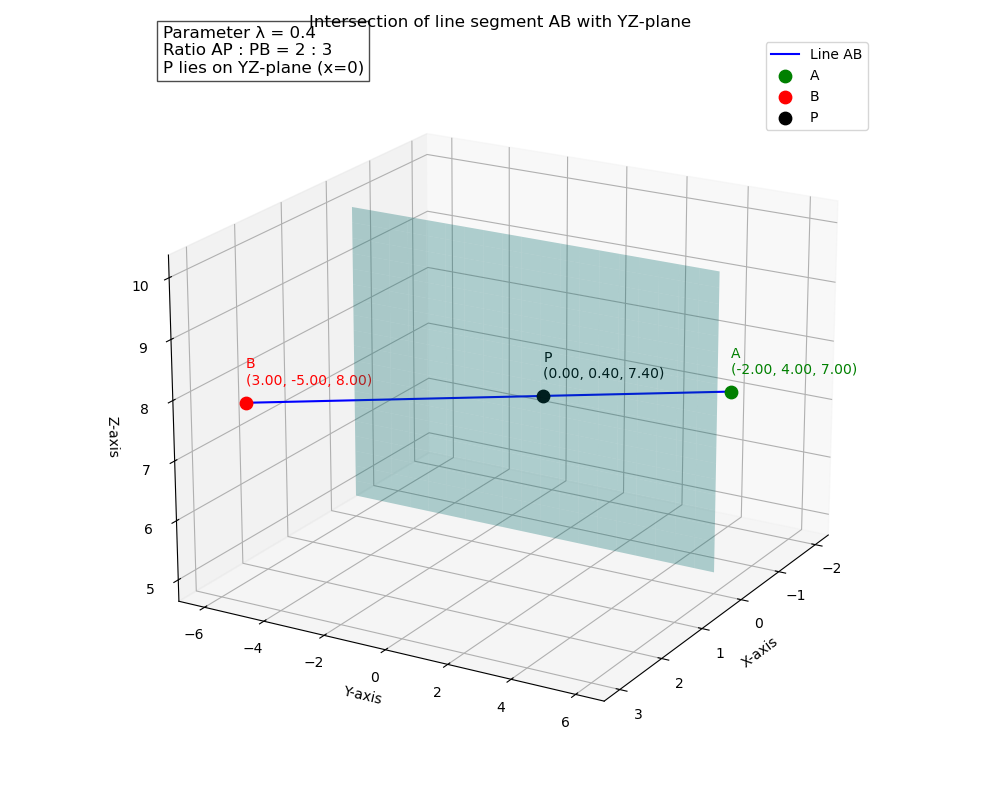
\includegraphics[width=0.9\columnwidth]{figs/fig_61.png}
    \caption{}
    \label{fig:placeholder}
\end{figure}
\end{frame}
\begin{frame}[fragile]{PLOTS}
\begin{figure}
    \centering
    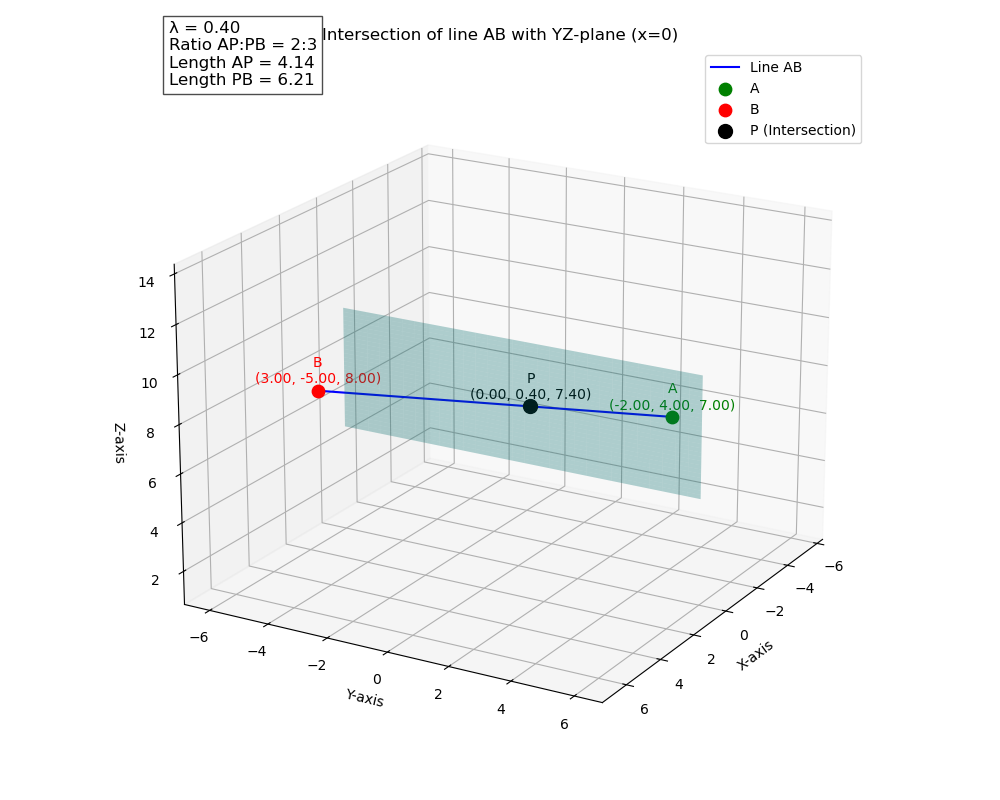
\includegraphics[width=0.9\columnwidth]{figs/Fig -62.png}
    \caption{}
    \label{fig:placeholder}
\end{figure}
\end{frame}
\end{document}
